\chapter{Opis projektnog zadatka}
		
		\section{Opis problema i motivacija}
		
			{Jedan je od glavnih problema života u studentskom domu pranje rublja. Studenti smješteni u domove
			moraju paziti na raspored pranja više nego na rokove za prijavu ispita, jer što im znači prijavljen ispit ako
			na njega nemaju u čemu doći. Motivacija za izradu ove web aplikacije leži u nepraktičnom sustavu
			rezerviranja termina pranja odjeće. Često se zna dogoditi da se student dođe upisati, ali naiđe na
			zatvorena vrata zbog pauza koje su stalno u drugo vrijeme ili nađe kompletno popunjen kalendar te ne
			može oprati veš. Želimo da se to iskustvo olakša studentima, ali i zaposlenicima praonice. Na ovaj bi se
			način mogli puno jednostavnije rezervirati, ali i otkazati termini za pranje koji bi se onda lako popunili te
			bi se studenti mogli puno bolje organizirati pa čak i upisati za termin koji je netom otkazan.
			Moderniziralo bi se i plaćanje te penaliziralo često otkazivanje dragocjenih termina.}
		
		\section{Postojeća slična rješenja}
		
			{Istraživanjem tržišta, zaključili smo da postoji nekoliko aplikacija koje se bave navedenim problemima.
			Jedna je od aplikacija koju smo uspjeli pronaći, a da je slična onome što želimo proizvesti slijedeća:
			\url{https://play.google.com/store/apps/details?id=net.celestialdata.ujlaundry&hl=en_US} (Slika  \ref{fig:ujlaundry}). Ta je aplikacija
			razvijena za praonicu na University of Jamestown-u. Dakako, razlika je u tome što je ovo isključivo
			mobilna aplikacija (postoje verzije za Android I IOS), a mi bismo napravili responzivnu web aplikaciju lako
			dostupnu svima s bilo kojeg uređaja koji ima pristup internetskoj mreži. Također, imamo I neke dodatne
			funkcionalnosti koje su navedene u usporedbi sa slijedećom aplikacijom (posudba košare, recenzije
			radnika, objava slika, oglasi za posao... ).}
		
			\begin{figure}[H]
				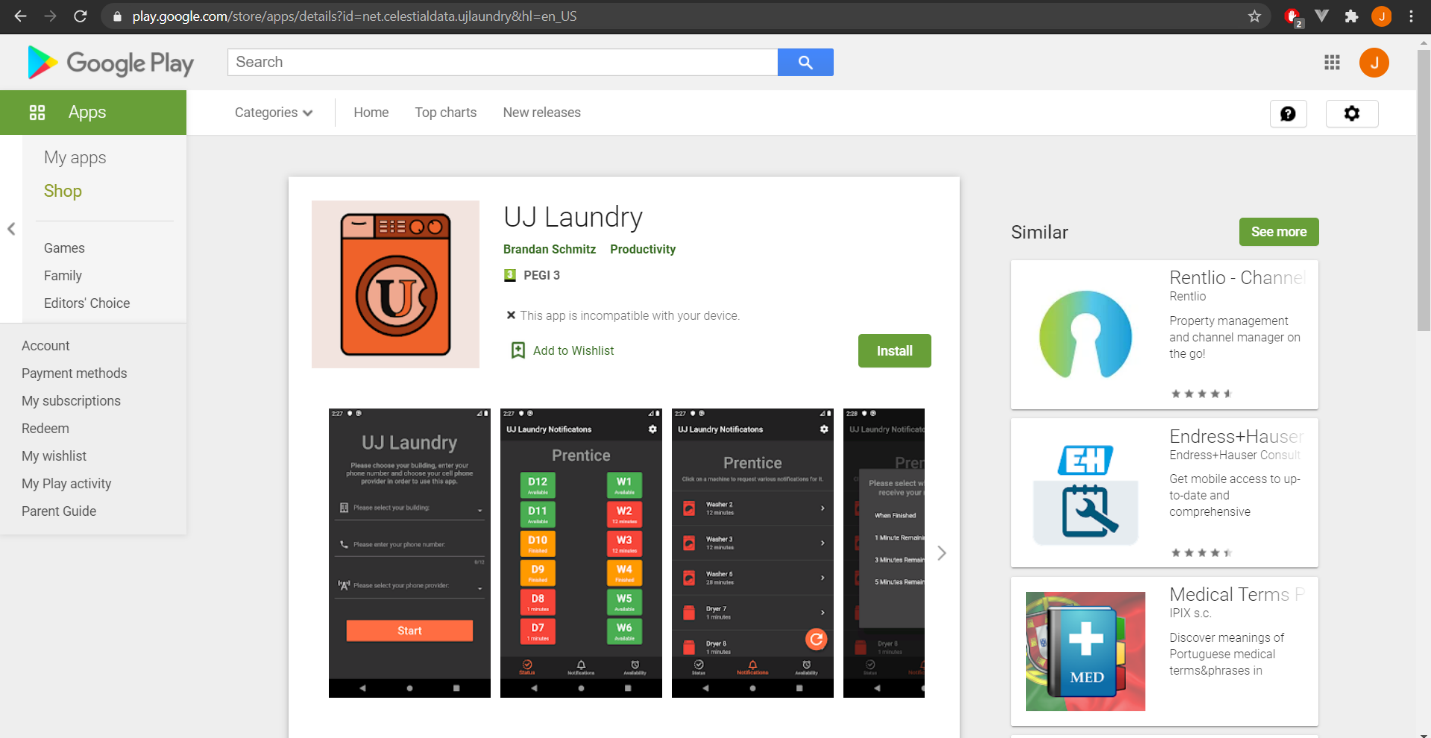
\includegraphics[width=.9\linewidth]{slike/UJLAUNDRY.PNG}
				\caption{Slika aplikacije "UJLAUNDRY"}
				\label{fig:ujlaundry}
			\end{figure}
		
			{Također, pronašli smo I slijedeću aplikaciju Nizozemskog porijekla: \url{https://www.duwo.nl/en/irent/residence-matters/washing-machine-with-a-qr-code} (Slika  \ref{fig:duwo}). Ta je aplikacija po glavnoj funkcionalnosti 
			poprilično slična našoj (web aplikacija koja omogućuje online rezervaciju termina i plaćanje preko
			interneta. Razlike su u tome što bi naša aplikacija bila prilagođenija studentskim domovima. Nudila bi
			funkcionalnost označavanja osobe koja je posudila košaru, recenzije radnika u praoni (što druge
			aplikacije nemaju jer su većinom vešeraju samoposlužni, duk je u domu zaposlen radnik), mogućnost
			objavljivanja slika izgubljenih stvari, mogućnost administratora da objavi oglas za posao u praoni, te
			mogućnost promijene radnog vremena, odnosno vremena pauzi na dnevnoj bazi. Također, ta aplikacija
			nema mogućnost slanja obavijesti na mail (npr. 1h prije početka termina).}
		
			\begin{figure}[H]
				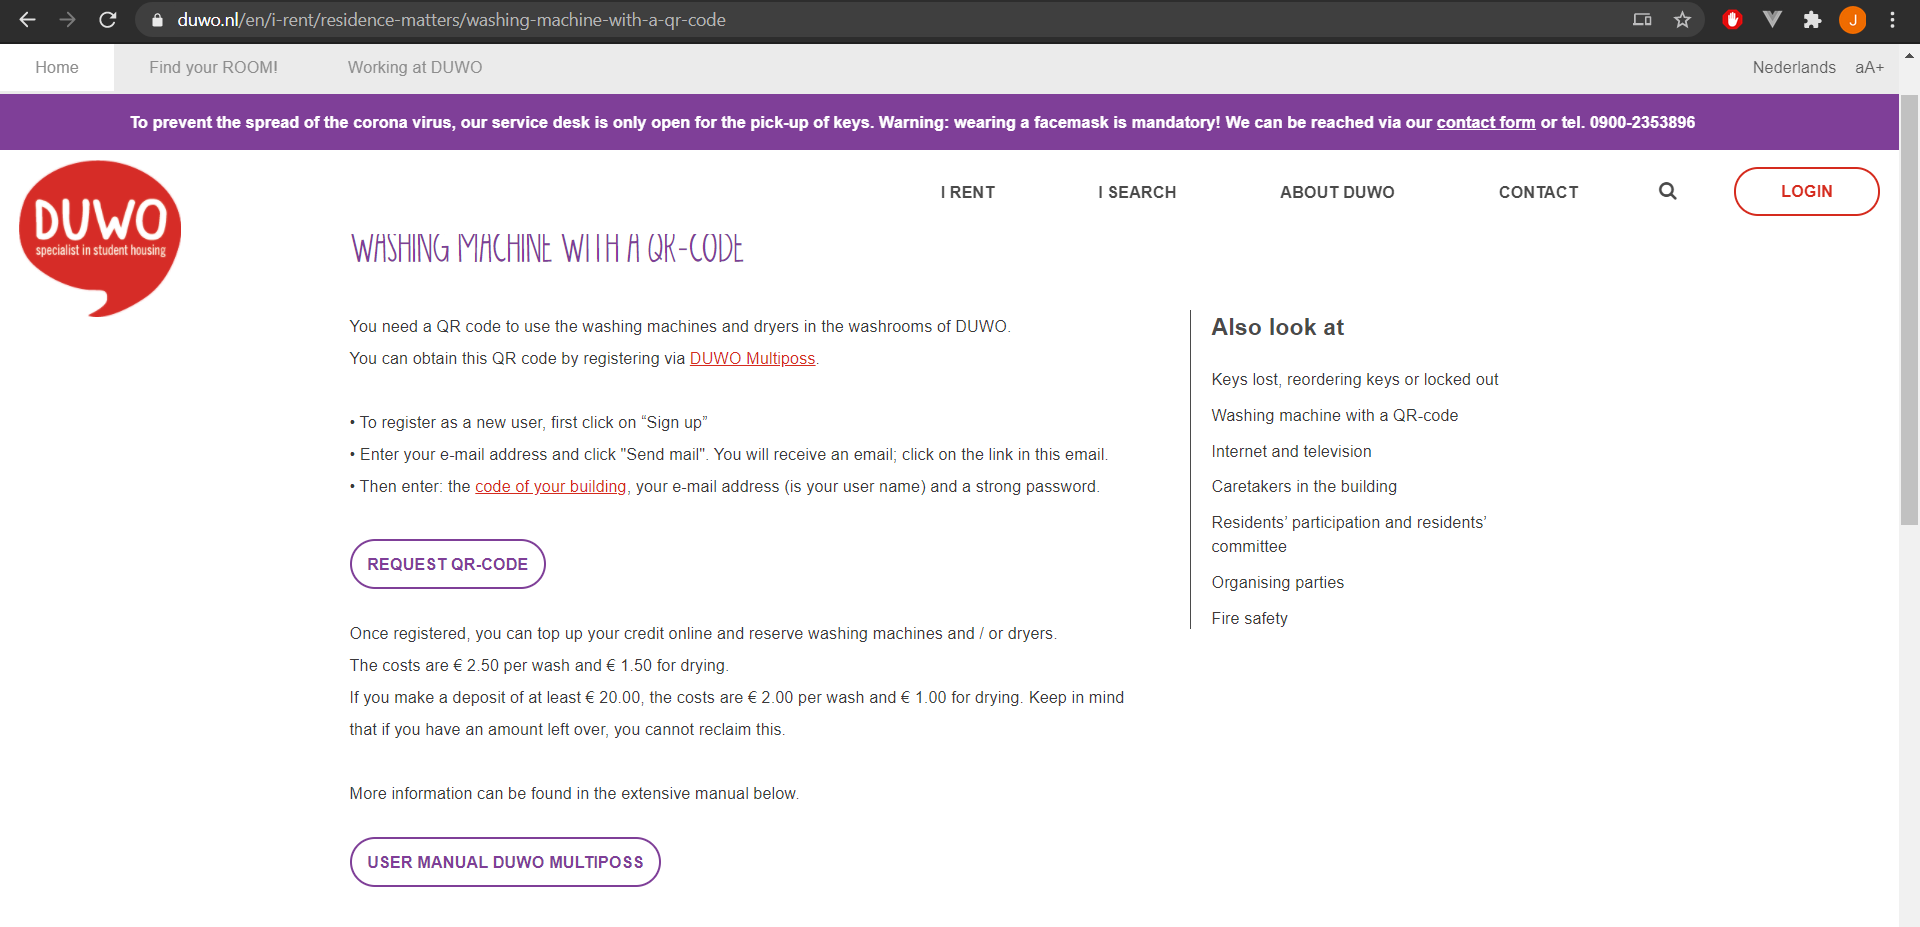
\includegraphics[width=.9\linewidth]{slike/DUWO.PNG}
				\caption{Slika aplikacije "Washing machine with a QR code"}
				\label{fig:duwo}
			\end{figure}
		
			{Treća pak stranica koju smo pronašli dolazi iz Norveške (Slika  \ref{fig:sit}). Sličnih je funkcionalnosti kao i prethodno
			navedena Nizozemska aplikacija, osim što ima dodatnu funkcionalnost, a to je slanje sms poruka za
			obavijesti (razlika u odnosu na našu je što bi mi slali na mail). Što se razlika tiče, slične su kao i u gore
			navedenom primjeru, uz razliku u tome što ova aplikacija, kao i naša, implementira slanje obavijesti
			korisnicima. }
		
			\begin{figure}[H]
				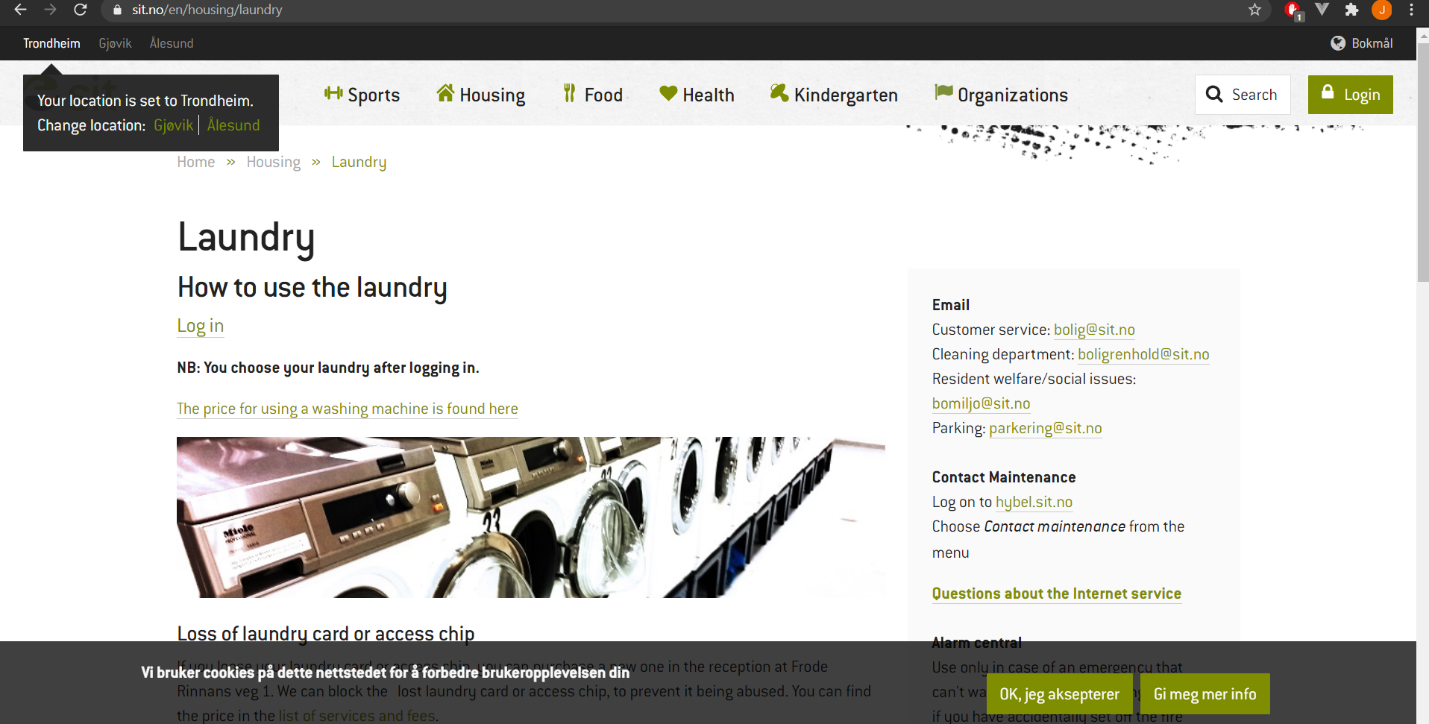
\includegraphics[width=.9\linewidth]{slike/SIT.PNG}
				\caption{Slika aplikacije za rezervaciju termina iz Norveške}
				\label{fig:sit}
			\end{figure}
		
			{Postoji i još nekoliko aplikacija sličnoga karaktera, no naveli smo 3 najpopularnije. Većina ostalih
			aplikacija dijele slične razlike u usporedbi s našom kao i gore navedene pa bi bilo redundantno navoditi
			ih.}
			
		\section{Potencijalno zainteresirani korisnici}
			
			{Za ovaj projekt očekujemo da će najveći interes pokazati studentski domovi s obzirom da je cilj projekta
			olakšavanje poslovanja već postojećih praonica veša u sklopu domova. No unatoč prvobitnom
			usmjerenju projekta prema studentskim domovima, smatramo da je ovakvo rješenje također opće
			primjenjivo i na ostale javne praonice jer primjenom ovakvog rješenja sa mogućnošću online rezervacije
			termina korisnik ne bi morao riskirati dolazak u punu praonicu te bi mogao izbjeći nepotrebno čekanje.
			Projekt bi također bilo moguće uvesti u ostale ustanove koje nude mogućnosti pranja veša kao što su
			npr. hoteli, kampusi itd.}	
		
		\section{Mogućnost prilagodbe rješenja}
			
			{Kao što smo već naveli gore, projekt se vrlo lako može prilagoditi potrebama krajnjeg korisnika pa tako u
			vidu imamo i potrebne prilagodbe za javne praonice veša kao i mogućnost izvoza proizvoda van hrvatske
			s obzirom da u planu imamo ponuditi i cijelu web aplikaciju na engleskom jeziku. Mogućnost izbora
			jezika također bi olakšala upotrebu aplikacije stranim studentima koji borave u hrvatskim studentskim
			domovima.}
			
		\section{Opseg projektnog zadatka (zahtjevi sustava)}
		
			{Korisnici ove aplikacije su: osoblje u SC-u zaduženo za rad praonice rublja u ulozi administratora,
			studenti, osobe zaposlene u praonici i neregistrirani korisnici.
			Neregistrirani korisnici u mogućnosti su samo napraviti svoj korisnički račun, vidjeti oglase za posao i
			radno vrijeme te nemaju mogućnosti ni za kakvu drugu radnju.
			Administratori (osoblje u SC-u zaduženo za rad praonice) jedini mogu postaviti oglas za posao u praonici
			na koji se mogu prijaviti ljudi koji su registrirani u aplikaciji. Oni također mogu mijenjati radno vrijeme
			praonice te zabilježiti eventualne promijene cijena pranja i sušenja rublja. Ako je potrebno,
			administrator može i blokirati pristup aplikaciji bilo kojem korisniku.
			Sljedeća su kategorija korisnika osobe zaposlene u praonici. Te osobe, poput administratora, mogu
			mijenjati radno vrijeme praonice te pauze. S obzirom da se termini za pranje i sušenje veša mogu
			rezervirati svakih 1:30h vremena (npr. ako praonica radi od 8, onda su mogući termini 8, 9:30, 11,
			12:30...), pauze mogu trajati maksimalno jedan sat (između 2 termina) te se nikako ne smije dogoditi da
			pauza bude kad je vrijeme zamjene veša. U aplikaciji osoba koja trenutno radi može označiti da je netko
			posudio košaru za veš i ako ne vrati zna se kod koga je. Također, ako osoba ne dođe pokupiti svoj veš,
			može mu poslati obavijest na mail da je veš gotov.
			Posljednja su vrsta korisnika ove aplikacije studenti. Oni će se moći prijaviti svojim AAI eduHr računom
			ako nam CARNET dozvoli korištenje AAI eduHr prijave, dok će u suprotnom moći napraviti korisnički
			račun te će morati čekati da im osobe zaposlene u praonici potvrde račun (nakon slanja zahtjeva za
			izradu računa morat će doći osobno u praonicu kako bi im osoba koja trenutno radi potvrdila račun).
			Glavna je funkcionalnost za ovu vrstu korisnika mogućnost rezervacije i otkazivanja termina za pranje i
			sušenje veša. Njima je na naslovnoj stranici prikazan kalendar sa slobodnim i popunjenim terminima te
			lagano mogu odabrati vrijeme i datum za željenu rezervaciju. Prilikom rezervacije moguće je odabrati
			način plaćanja pranja – putem aplikacije ili na blagajni doma. Također, student može postaviti bilješku
			kod rezervacije npr. ne mogu doći po veš zbog obaveza na fakultetu, kasnit ću 2 sata. Termin se smije
			otkazati do 24 sata prije termina, a ako netko otkaže neposredno prije ili nakon termina za otkaz dobiva
			negativne bodove (ako se učestalo ponavlja korisnik je dužan platiti kaznu). Studentu će sat vremena
			prije njegovog termina na mail stići obavijest kako ne bi zaboravio doći ili otkazati termin.
			Studenti mogu i ocijeniti radnika u praoni nakon pranja veša i to samo onoga tko je bio u njihovom
			terminu jedanput po pranju.
			U ovoj će aplikaciji postojati i zid s objavama na kojem osoba zaposlena u praoni objavljuje slike
			izgubljenih stvari. Ako je stvar izgubljena dulje od mjesec dana objava se briše i stvar se donira u
			dobrotvorne svrhe. }
		
		\section{Nadogradnje projektnog zadatka i planovi za budućnost}
		
			{Moguća nadogradnja bi bila uključivanje više usluga koje se nude studentima u sklopu doma npr.
			rezervacija termina u teretani (koja ima ograničen broj mjesta I inače, a osobito sada u vrijeme
			pandemije), pregledi menija u menzi i radnog vremena, kupnja karti za Kino SC, Teatar \&TD i slično.
			Sljedeći korak u razvoju bi mogao biti razvoj mobilne aplikacije jer bi većina studenata sustavu pristupala
			na taj način. Nakon razvitka mobilne aplikacije, može se pristupiti izgradnji interaktivnog vodiča za
			brucoše. Vodič bi naše brucoše na licu mjesta mogao provesti kroz način funkcioniranja veš mašina,
			ponuditi im savjet koji program služi za njihovu robu, te bi se time smanjila interakcija između
			zaposlenika i studenta.
			Preinakama originalne aplikacije mogli bi ju ponuditi i ostalim samoposlužnim vešerajima po Hrvatskoj
			ali i svijetu. Morali bi istražiti koje su im funkcionalnosti bitne, a koje bi trebalo ukloniti u odnosu na
			aplikaciju specifičnu za vešeraje u studentskim domovima.}